% Created 2024-11-21 Thu 21:58
% Intended LaTeX compiler: xelatex

\documentclass[10pt]{beamer}

% fonts
\usepackage{ctex}
\usepackage{fontspec}
\setmainfont{Times New Roman}
\setmonofont{Inconsolata}
\setsansfont{Times New Roman}
\setCJKmainfont{SimSong} % much more beautiful than STSong, which is sans serif
\setCJKsansfont{SimSong}
\setCJKmonofont{LXGW WenKai Mono}

\usepackage{amsfonts}
\usepackage{amsthm}
\usepackage{bm}
\usepackage{siunitx}
\usepackage{xcolor}

\usepackage{mathrsfs}
% commands
\newcommand{\mr}[1]{\mathrm{#1}}
\newcommand{\mb}[1]{\mathbf{#1}}
\newcommand{\mc}[1]{\mathcal{#1}}
\newcommand{\ms}[1]{\mathscr{#1}}

\usepackage{graphicx}
\usepackage{longtable}
\usepackage{wrapfig}
\usepackage{rotating}
\usepackage[normalem]{ulem}
\usepackage{amsmath}
\usepackage{amssymb}
\usepackage{capt-of}
\usepackage{hyperref}
\usepackage{etoolbox}
\usepackage{pgfopts}
\usepackage{booktabs}
\usepackage[scale=2]{ccicons}
\usetheme[block=fill, progressbar=frametitle]{metropolis}
\useoutertheme{infolines} % infoline
\useinnertheme{default}
\usecolortheme{custom} % custom color theme
\setbeamertemplate{blocks}[rounded][shadow=false]
\setbeamertemplate{items}[circle] % circle item symbol
\setbeamertemplate{sections/subsections in toc}[ball] % ball section symbol
\setbeamertemplate{headline}[default] % no infoline headline
%\setbeamertemplate{footline}[default] % infoline footline
\setbeamertemplate{frame numbering}[none]
\setbeamertemplate{bibliography item}[text] % text references
%\setbeamerfont{footnote}{\tiny} % tiny footnote
\usetheme{default}
\author{朱宇涛 \quad 报告人: 王亚朋}
\date{2024年 11 月 21日}
\title{能量刻度与飞行时间测量}
\subtitle{宇宙线粒子探测与物理实验}

\hypersetup{
pdfauthor={朱宇涛 \quad 报告人: 王亚朋},
pdftitle={能量刻度与飞行时间测量},
pdfkeywords={},
pdfsubject={},
pdfcreator={Emacs 29.1 (Org mode 9.6.6)},
pdflang={English},
colorlinks=true,
linkcolor=black
}
\begin{document}

\maketitle
\section{实验内容}
\label{sec:orgb85fb84}
\begin{frame}[label={sec:org39214a7}]{实验内容}
\begin{enumerate}
\item 单光子电荷与能量刻度;
\item 余波;
\item Michel 电子能谱与 \(\mu\) 寿命;
\item \(\mu\) 飞行时间.
\end{enumerate}
\end{frame}
\begin{frame}[label={sec:org2231b0d}]{实验装置}
\begin{figure}[htbp]
\centering
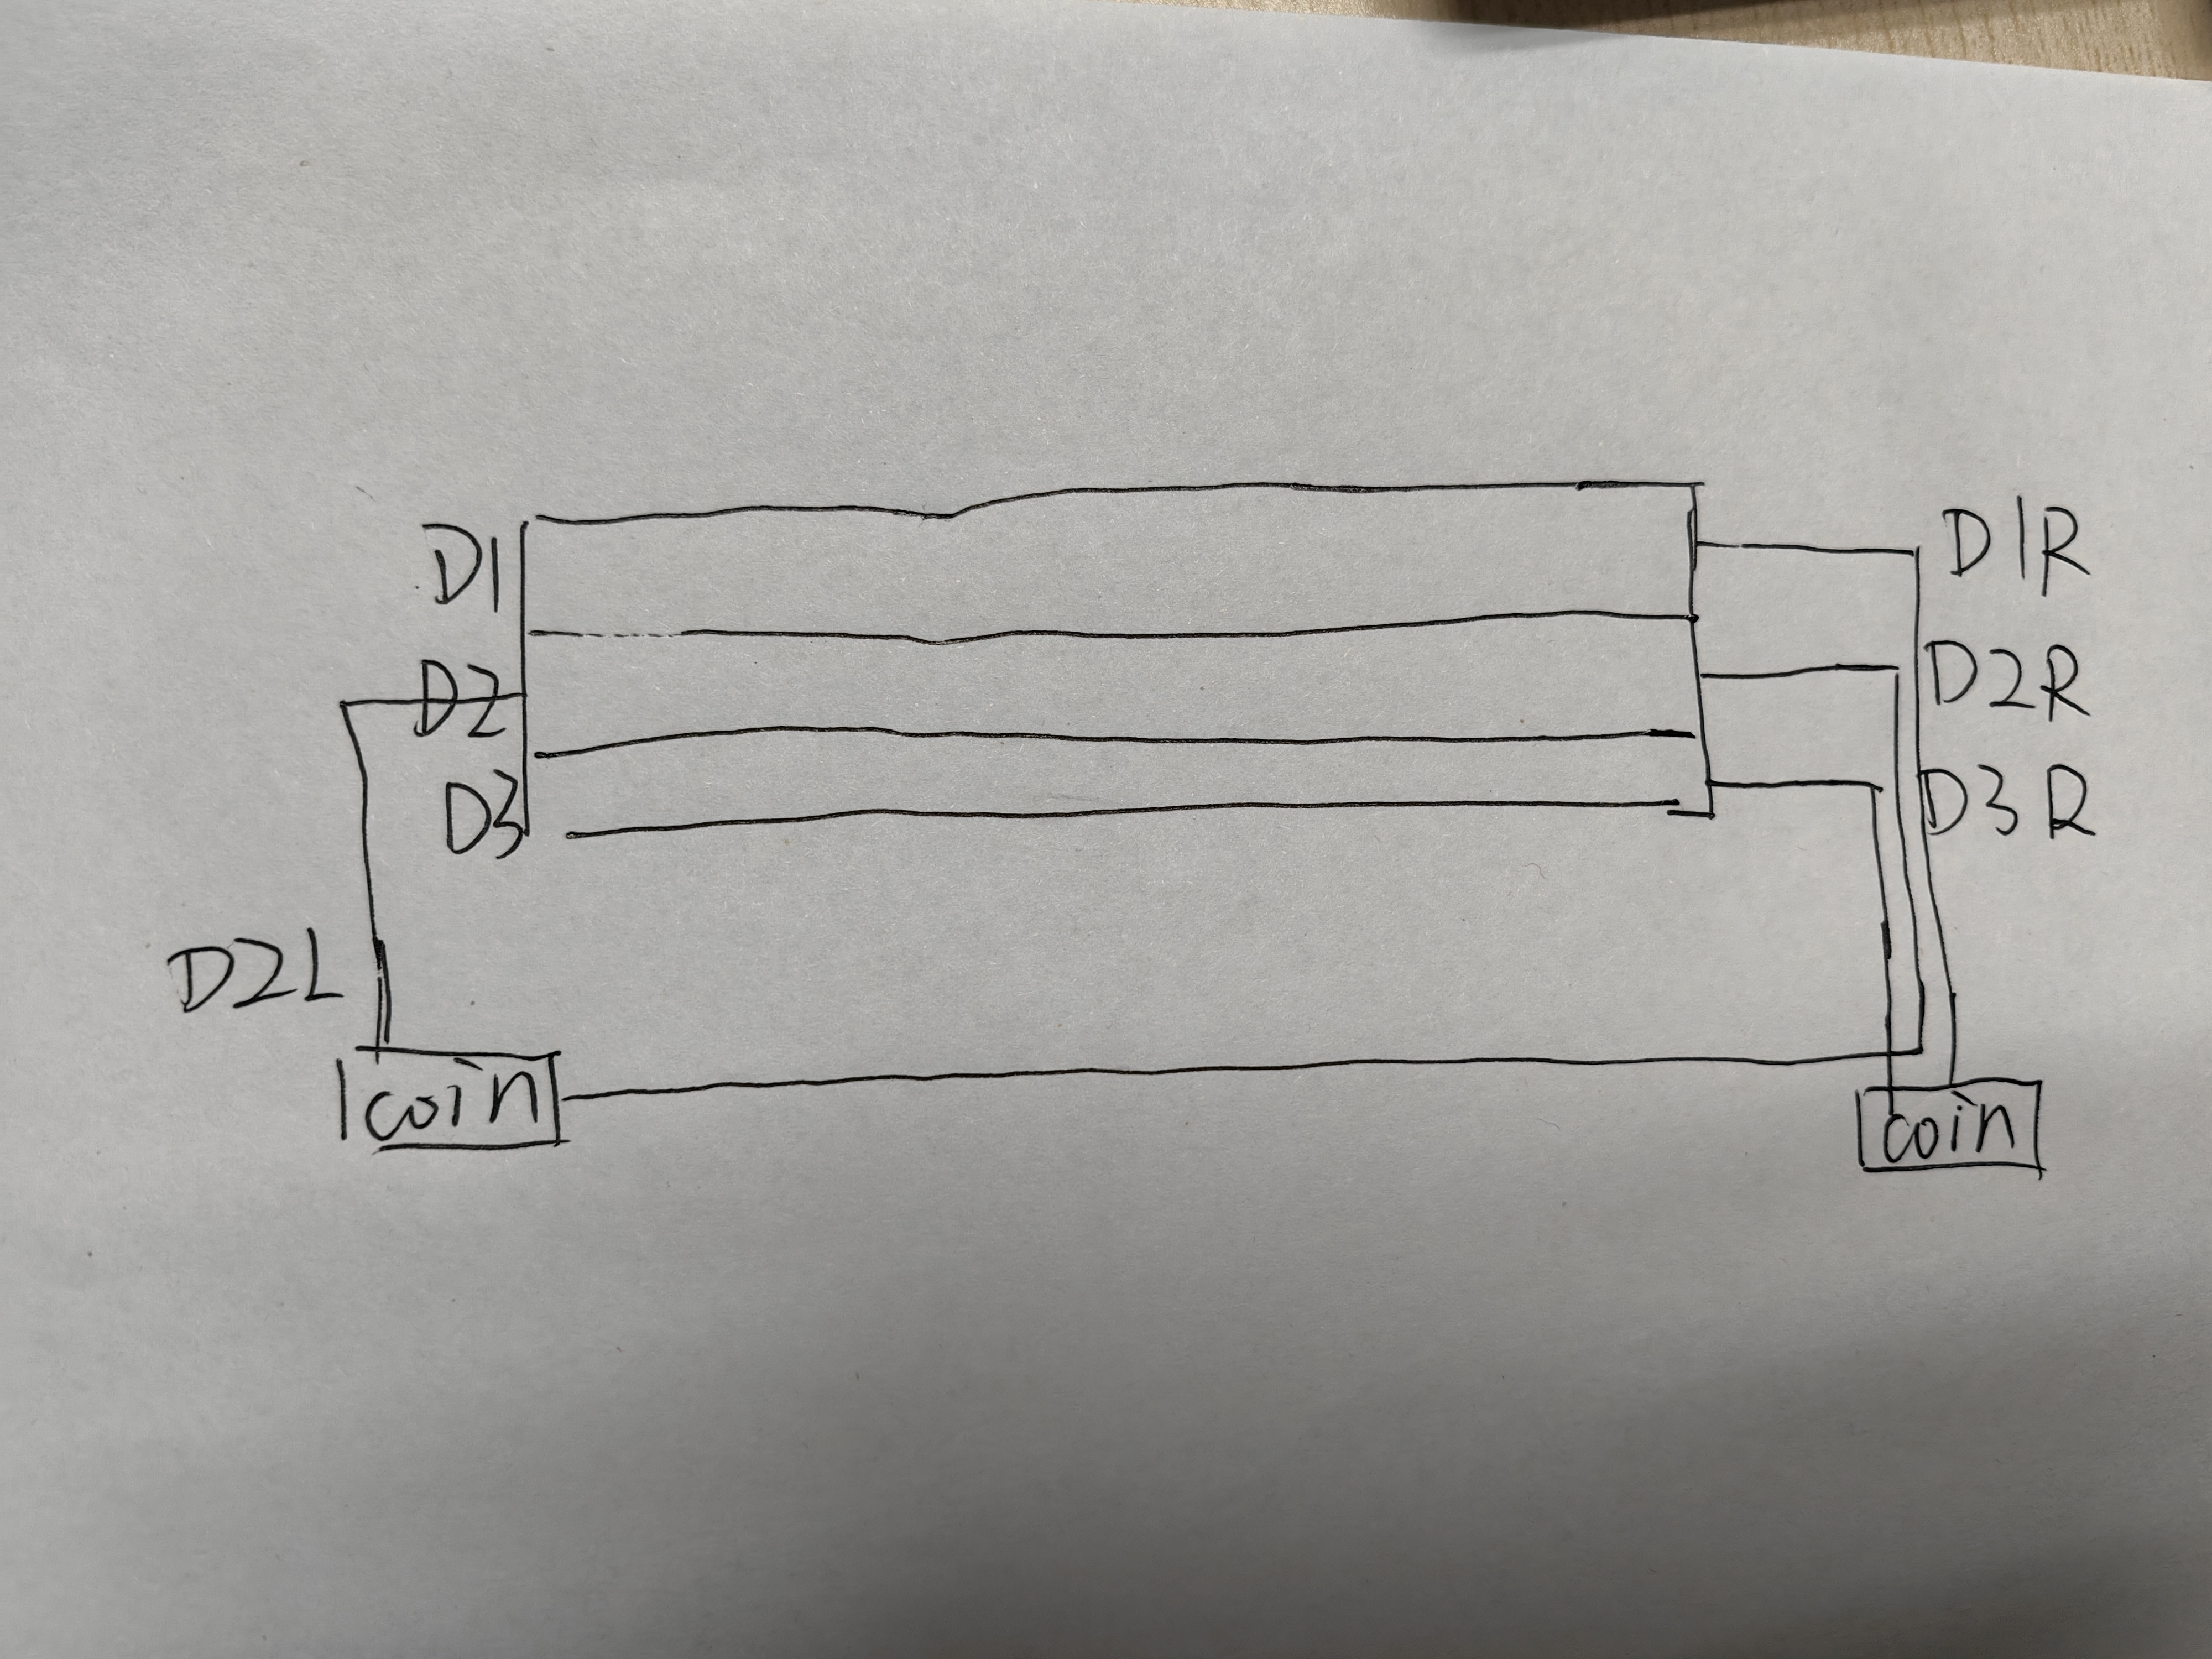
\includegraphics[width=0.6\textwidth]{../../img/instru.jpg}
\caption{实验装置}
\end{figure}
\end{frame}

\begin{frame}[label={sec:org1151998}]{单光子电荷}
在 4 路电压均为 1500V, 15mV 甄别阈下重新测量了单光子电荷.
\begin{figure}[htbp]
\centering
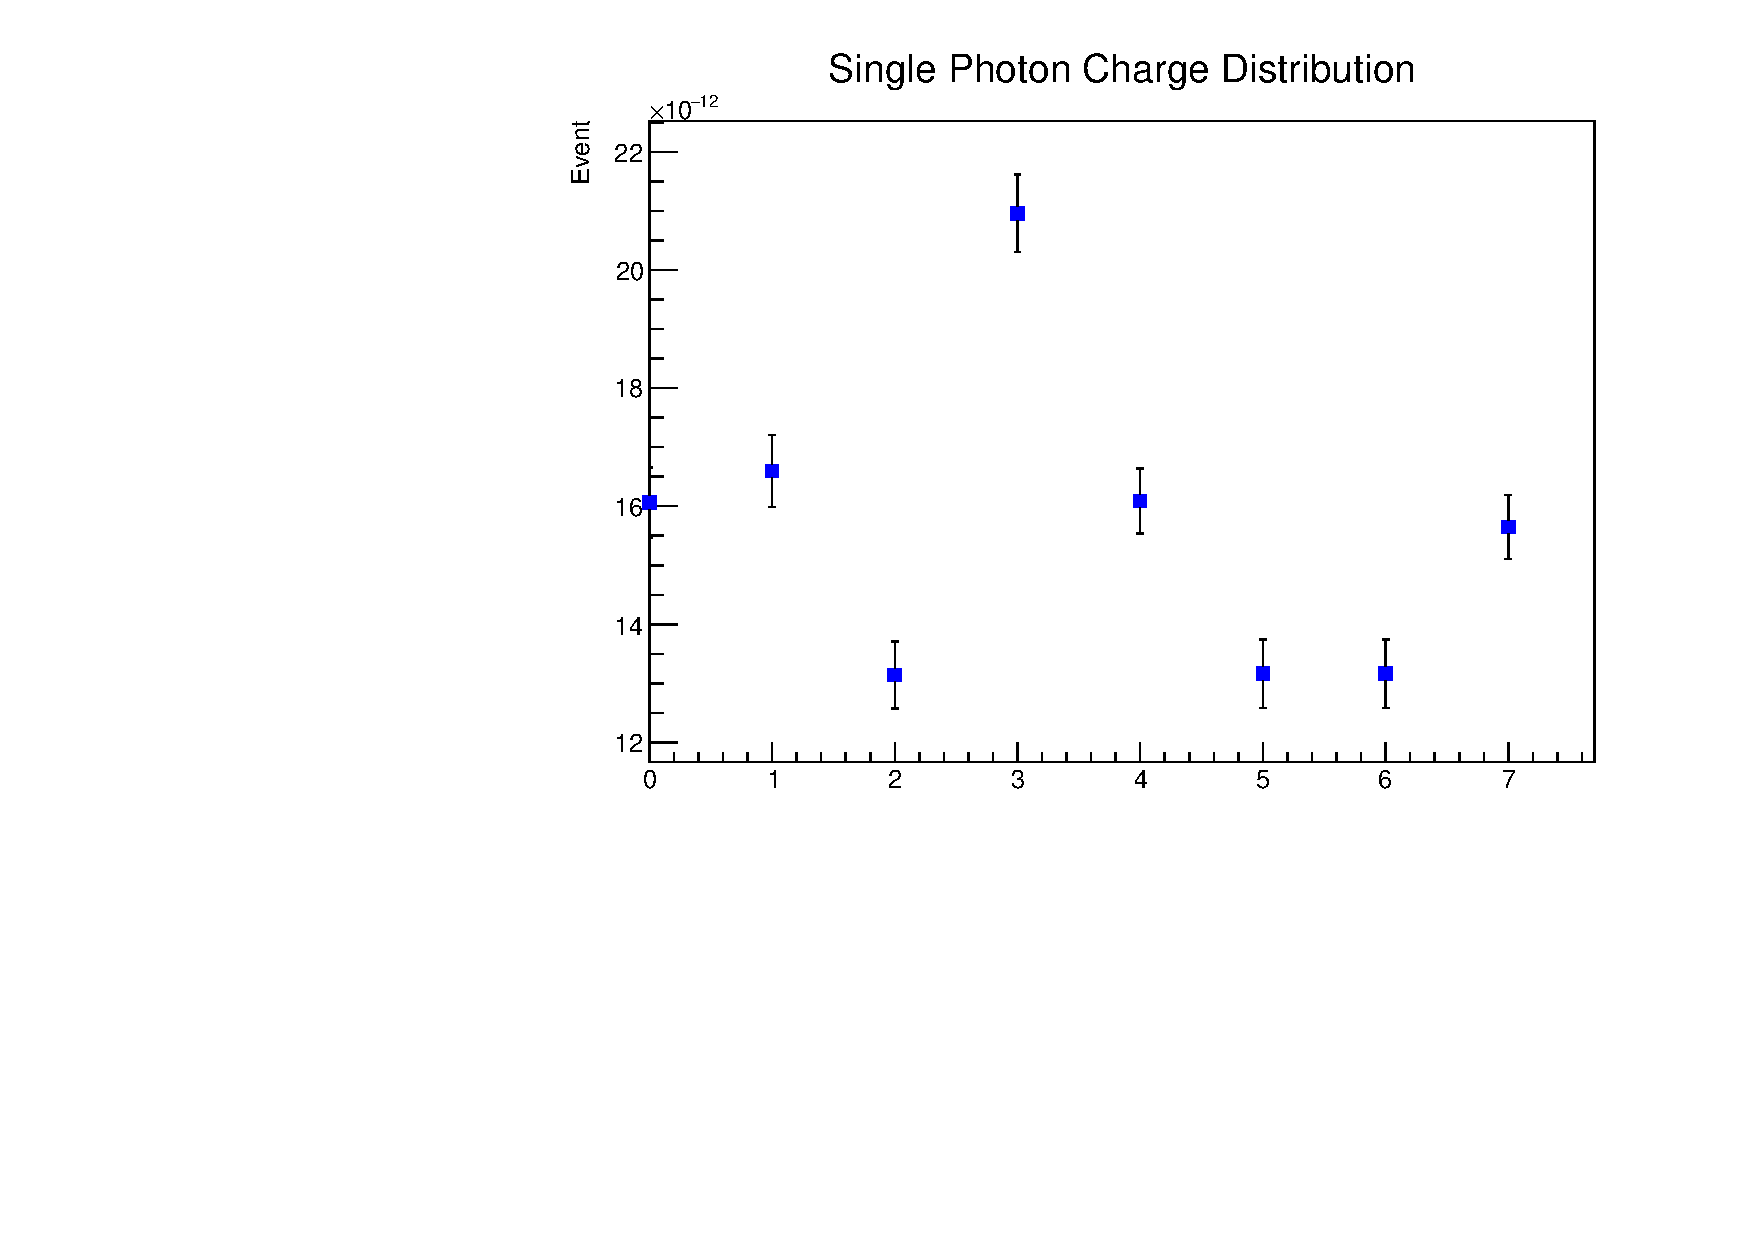
\includegraphics[width=0.5\textwidth]{../../DetectorPerform/SPhoton/SphotonCharge.pdf}
\caption{单光子电荷}
\end{figure}
根据 \(G = q/(Re)\) 计算得到:
\begin{itemize}
\item \(G_1 = (4.322 \pm 0.152) \times 10^7\).
\item \(G_2 = (1.887 \pm 0.097) \times 10^7\).
\end{itemize}
\end{frame}

\begin{frame}[label={sec:org251d697}]{能量刻度}
\begin{figure}[htbp]
\centering
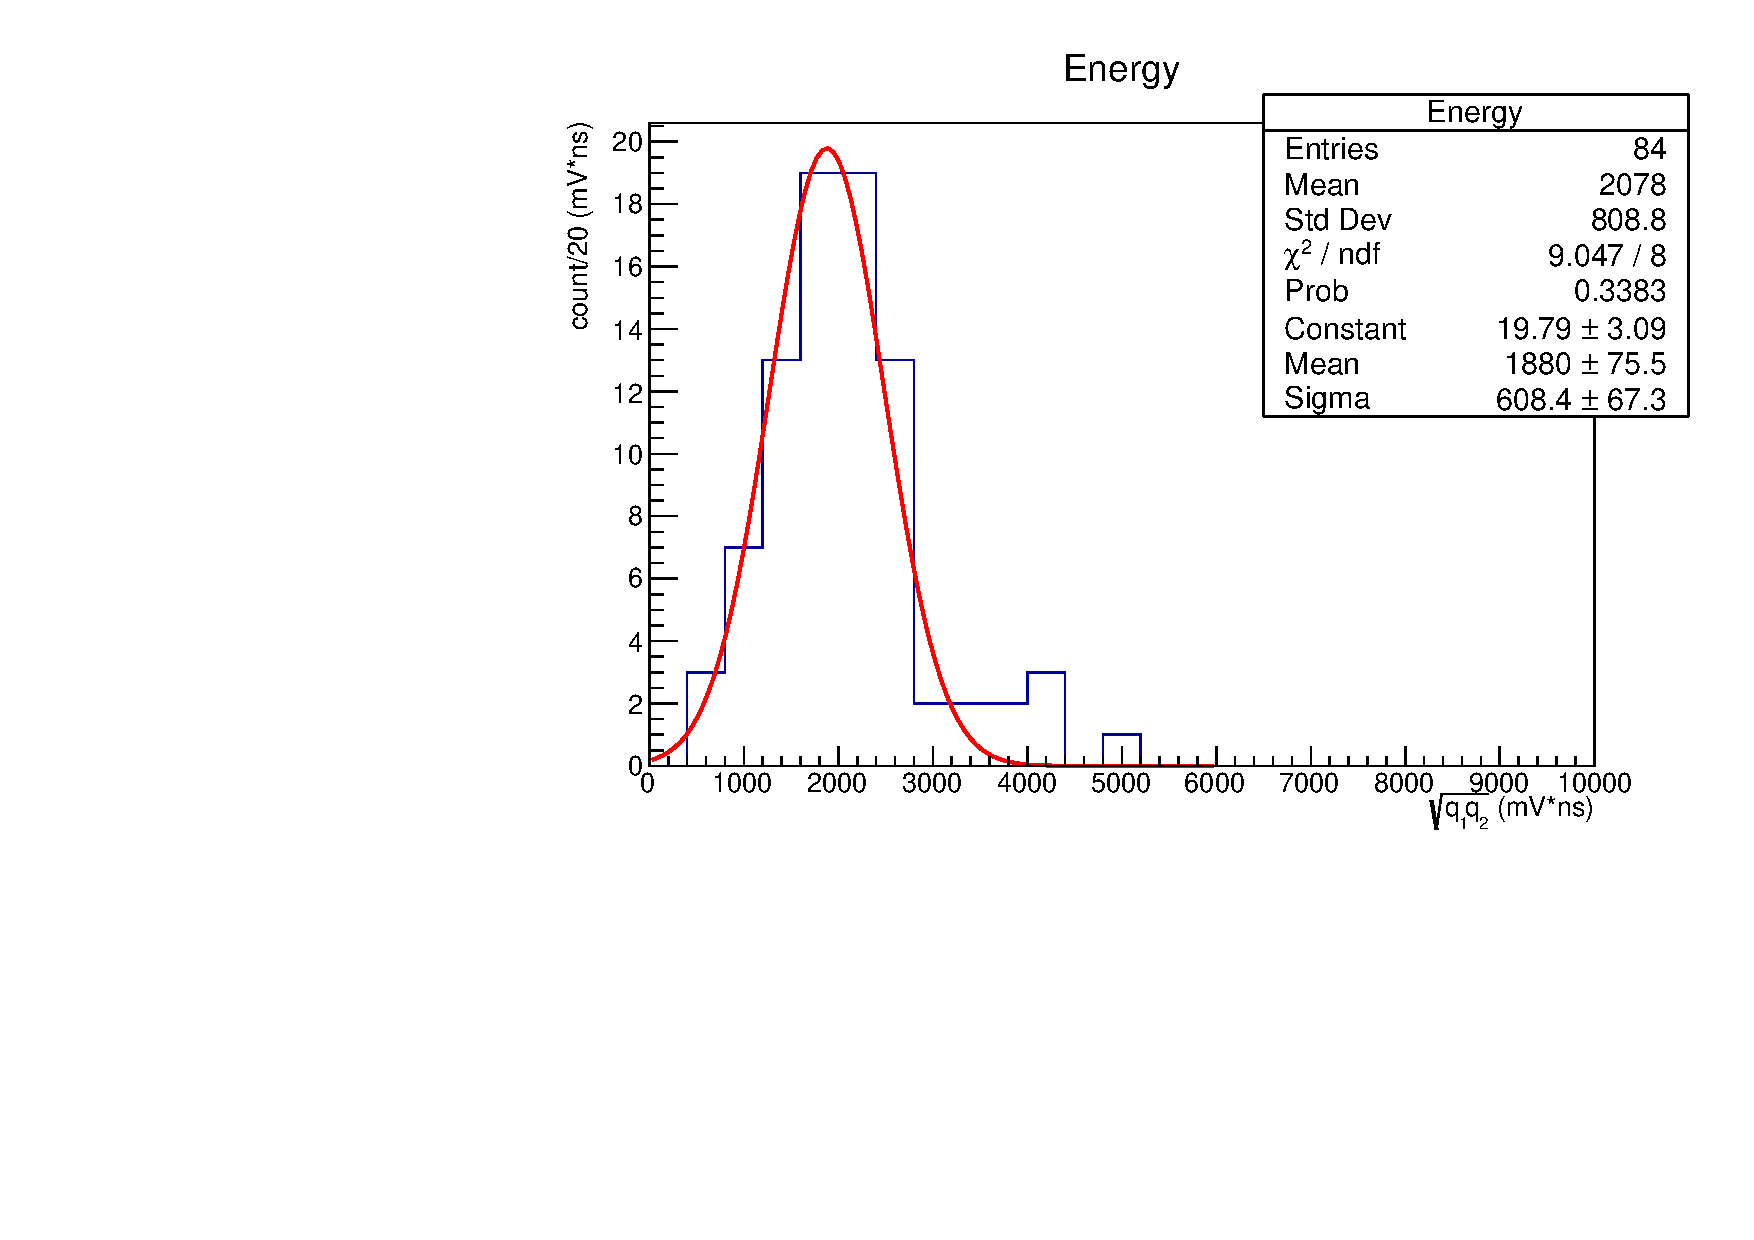
\includegraphics[width=0.5\textwidth]{../../DetectorPerform/ECali/qqEdist.pdf}
\caption{能量刻度}
\end{figure}
\begin{itemize}
\item 刻度系数: \(f = \qty{5.304e-3}{MeV \cdot mV^{-1} \cdot ns^{-1}}\).
\item 能量分辨率: 72.3\%.
\item 光产额: \(N = e^{L/2L_0} / (q f) = \qty{13.84}{MeV^{-1}}\)
\end{itemize}
\end{frame}

\begin{frame}[label={sec:org810d366}]{\(\mu\) 余波}
通过对 \(\mu\) 余波的测量得知:
\begin{itemize}
\item 出现余波的概率为 10\%;
\item 余波的时间分布集中在 0 \textasciitilde{} 3 \unit{\mu s};
\item 余波的幅值集中在 30 \textasciitilde{} 70 \unit{mV}.
\end{itemize}
\end{frame}

\begin{frame}[label={sec:orgde237ab}]{Michel 电子能谱}
在电压 1500V, 80mV 甄别阈\footnote{排除后脉冲.}条件下重新测量 Michel 电子能谱.
\begin{columns}
\begin{column}{0.5\columnwidth}
\begin{figure}[htbp]
\centering
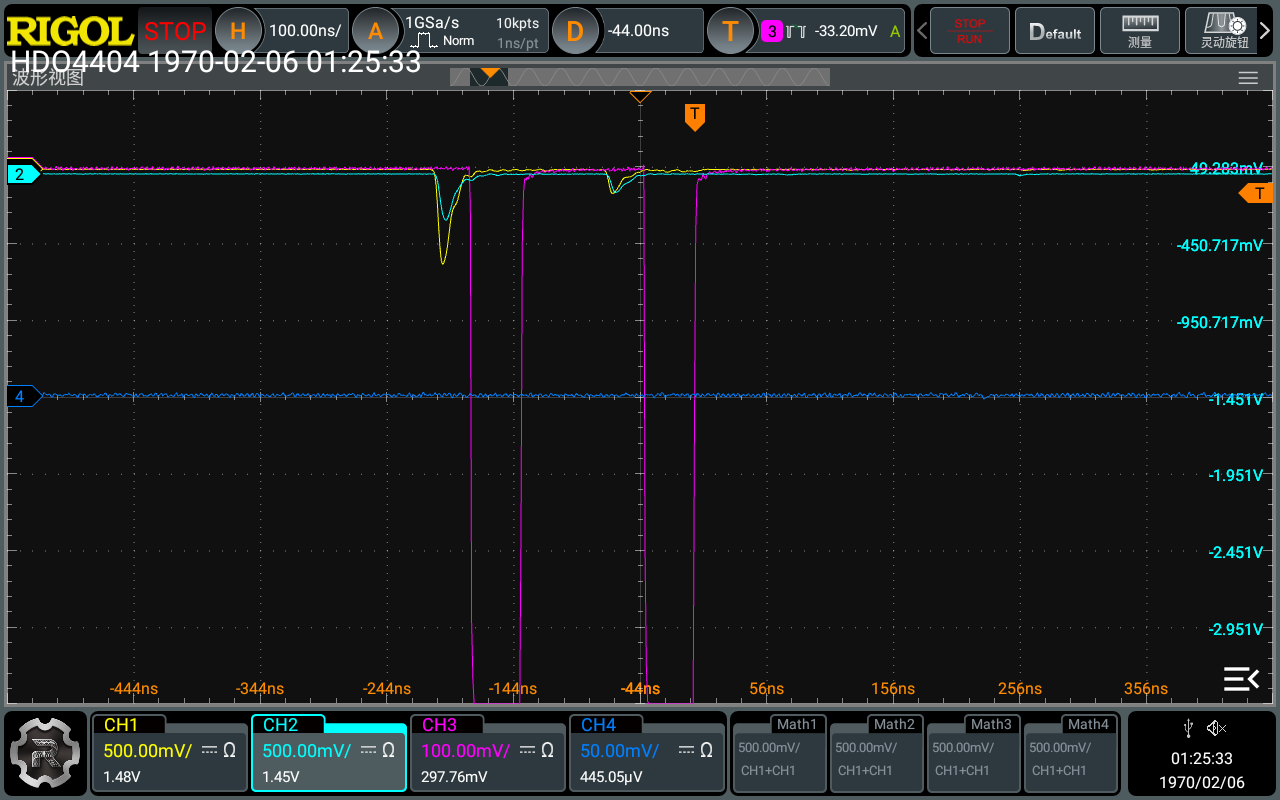
\includegraphics[width=0.9\textwidth]{../../ExperimentData/michel/michel/mudecay0.png}
\caption{典型信号}
\end{figure}
\end{column}

\begin{column}{0.5\columnwidth}
\begin{figure}[htbp]
\centering
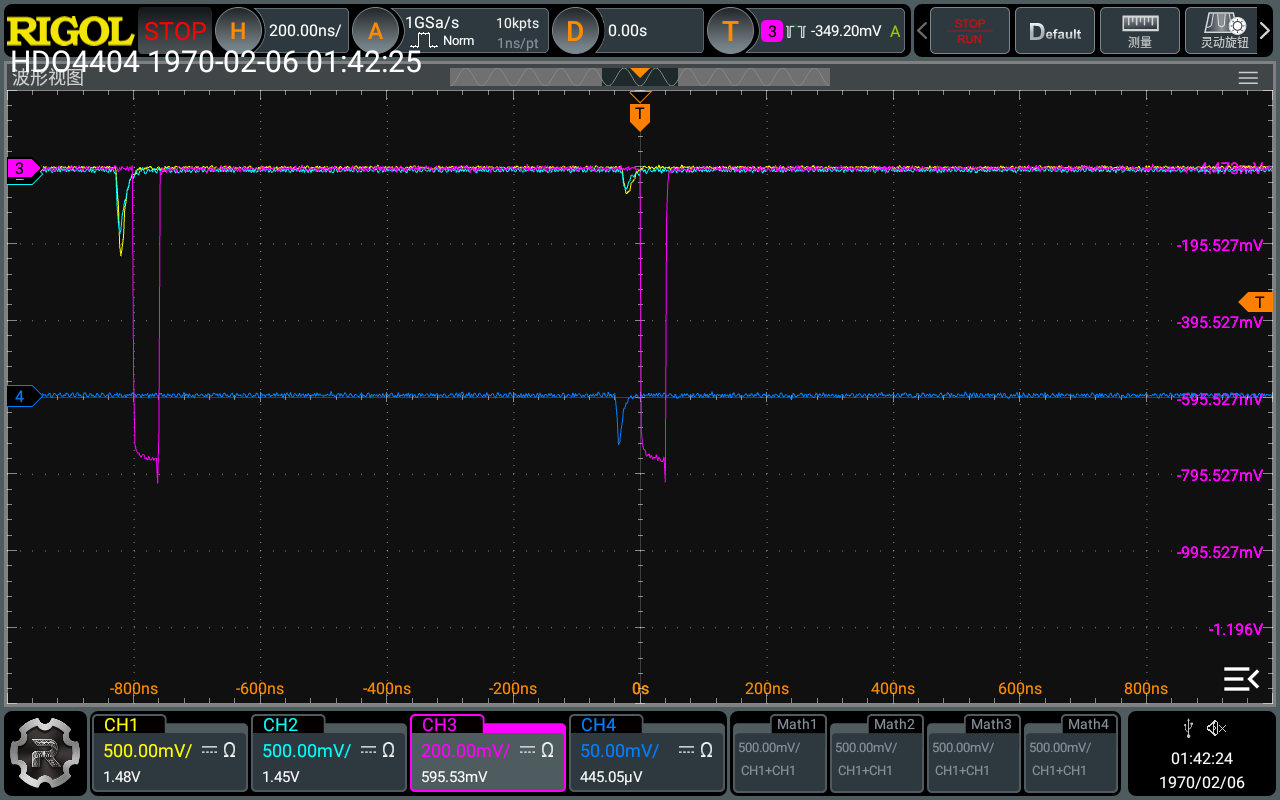
\includegraphics[width=0.9\textwidth]{../../ExperimentData/michel/michel/mudecay1.png}
\caption{特殊信号}
\end{figure}
\end{column}
\end{columns}
\end{frame}

\begin{frame}[label={sec:org10c2e4d}]{Michel 电子能谱}
\begin{figure}[htbp]
\centering
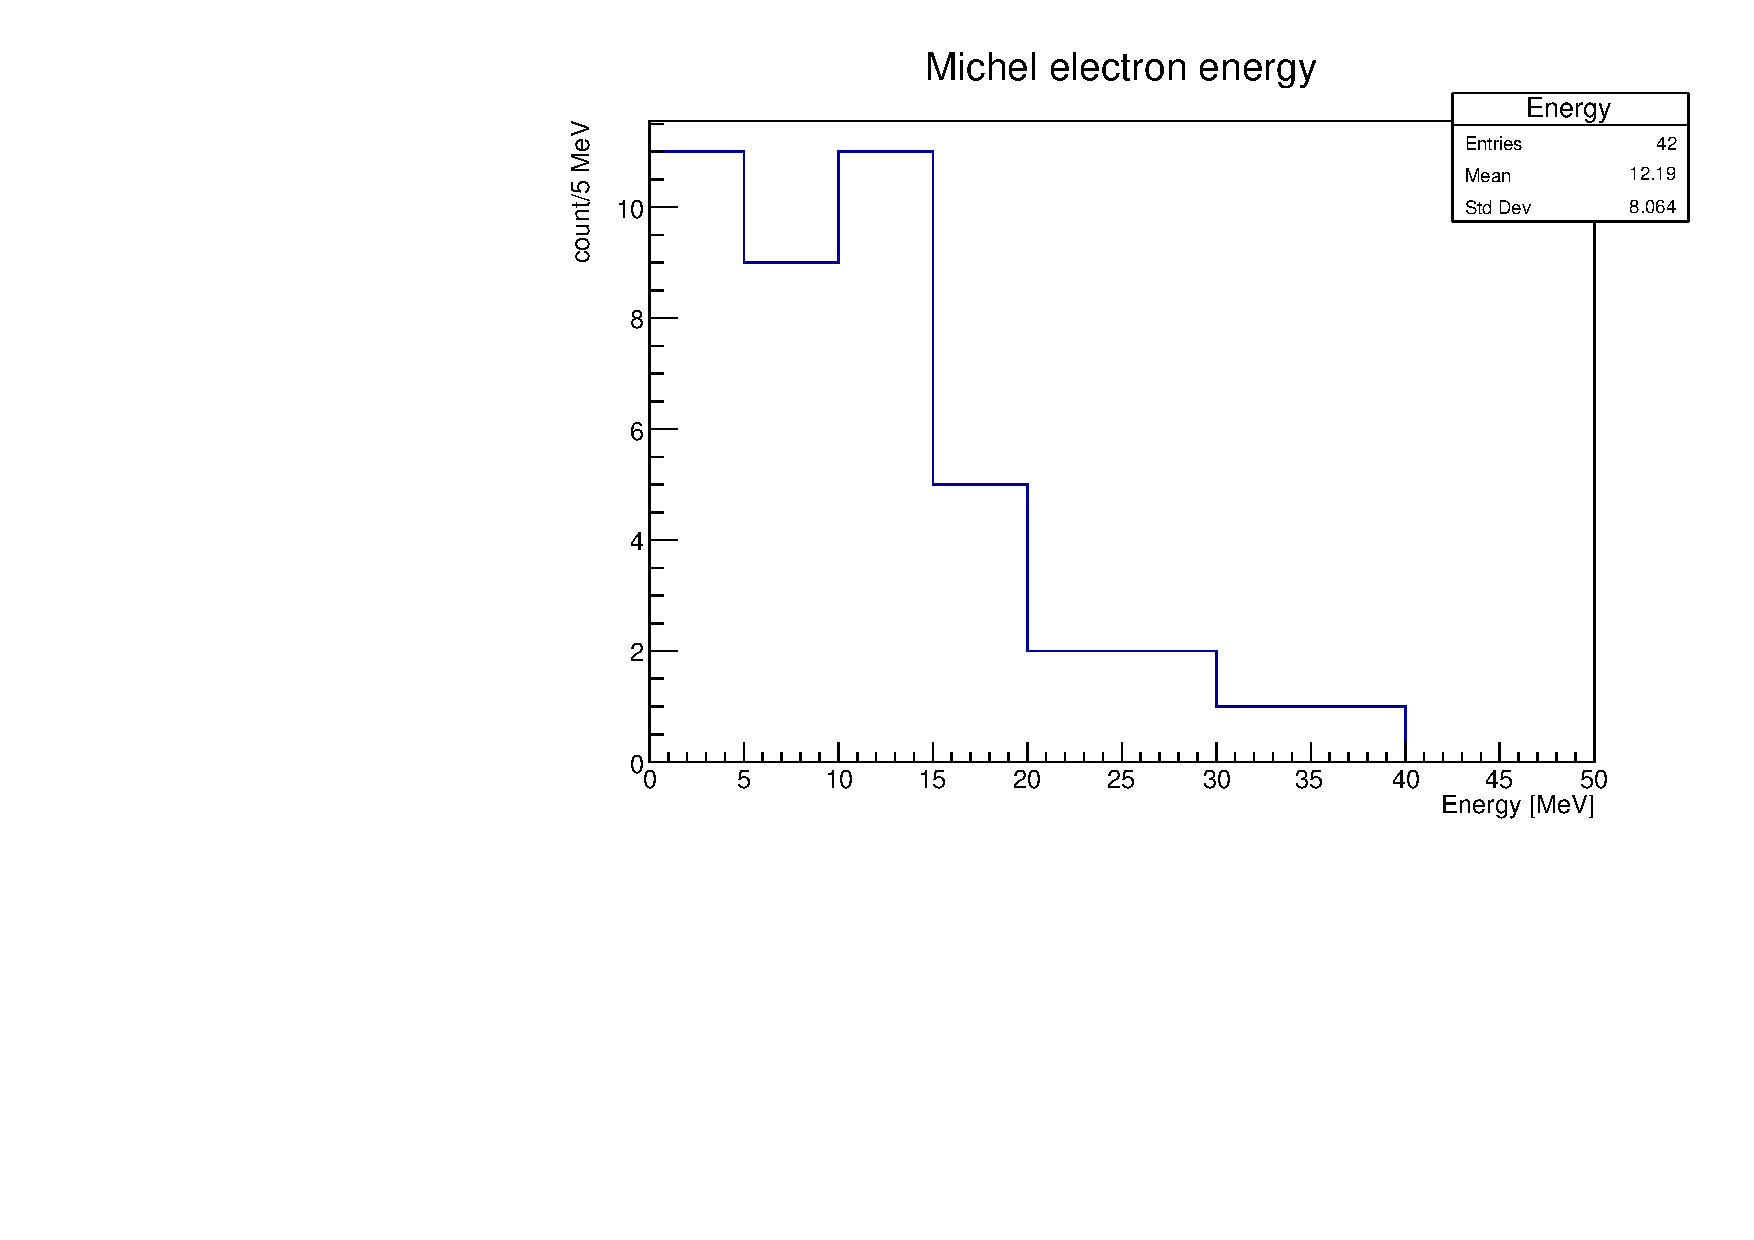
\includegraphics[width=0.5\textwidth]{../../mu/michel/michel.pdf}
\caption{Michel 电子能谱}
\end{figure}
能量最高达 50 MeV.
\end{frame}

\begin{frame}[label={sec:orgeaa717b}]{\(\mu\) 寿命}
\begin{columns}
\begin{column}{0.5\columnwidth}
\begin{figure}[htbp]
\centering
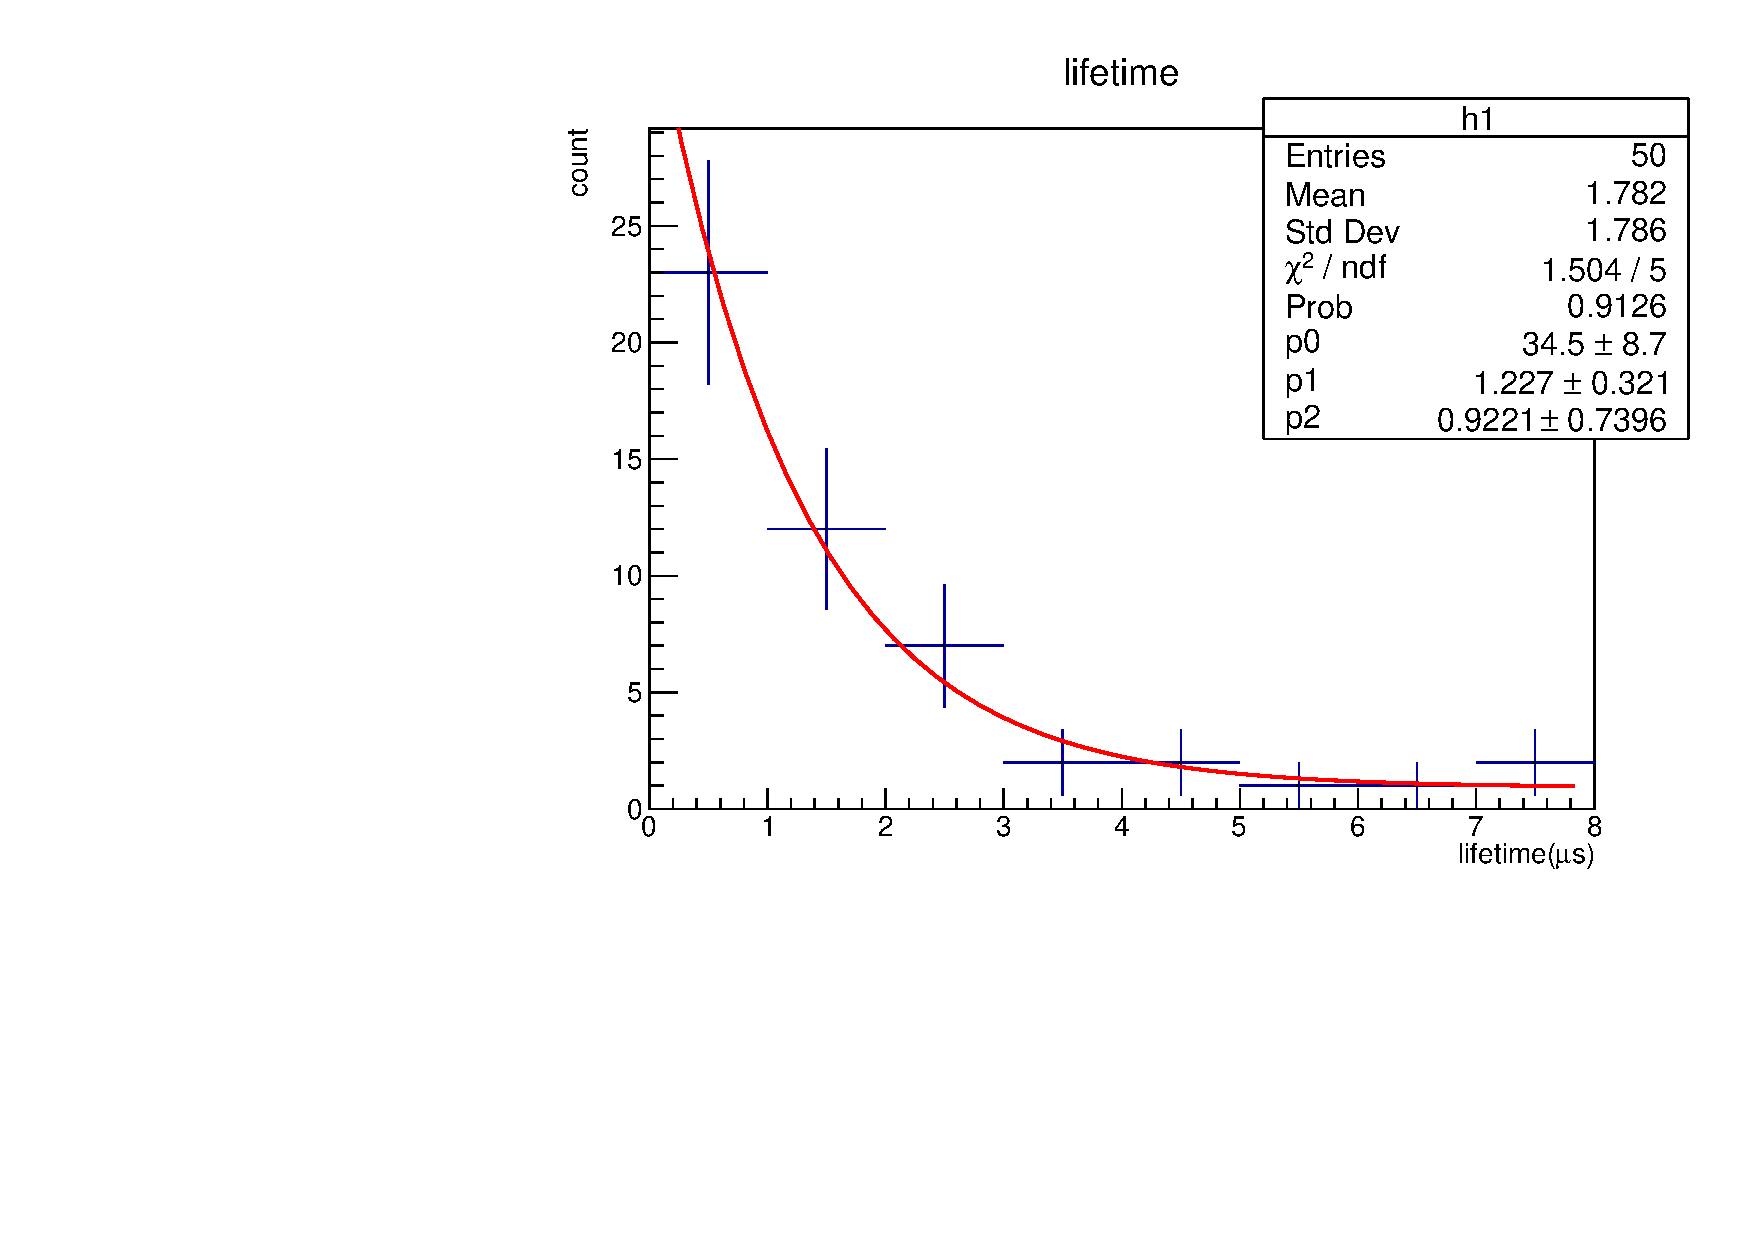
\includegraphics[width=0.9\textwidth]{../../img/lifeHist.pdf}
\caption{\(\mu\) 寿命}
\end{figure}
\end{column}
\begin{column}{0.5\columnwidth}
用 Michel 电子测量数据估计 \(\mu\) 寿命:
\[\tau_{\mu} = 1.227 \pm \qty{0.321}{\mu s}.\]
\end{column}
\end{columns}
\end{frame}

\begin{frame}[label={sec:orgdb3464a}]{飞行时间}
在两路电压为 1000V\footnote{右侧两闪烁体信号幅值较大, 故下调电压.}, 100mV 甄别阈下, 通过调整两闪烁体间距测量了 \(\mu\) 飞行时间.

\begin{itemize}
\item \(\mu\) 速度: \(v_{\mu} = (0.85 \pm 0.07) c\).
\end{itemize}

\begin{columns}
\begin{column}{0.5\columnwidth}
\begin{figure}[htbp]
\centering
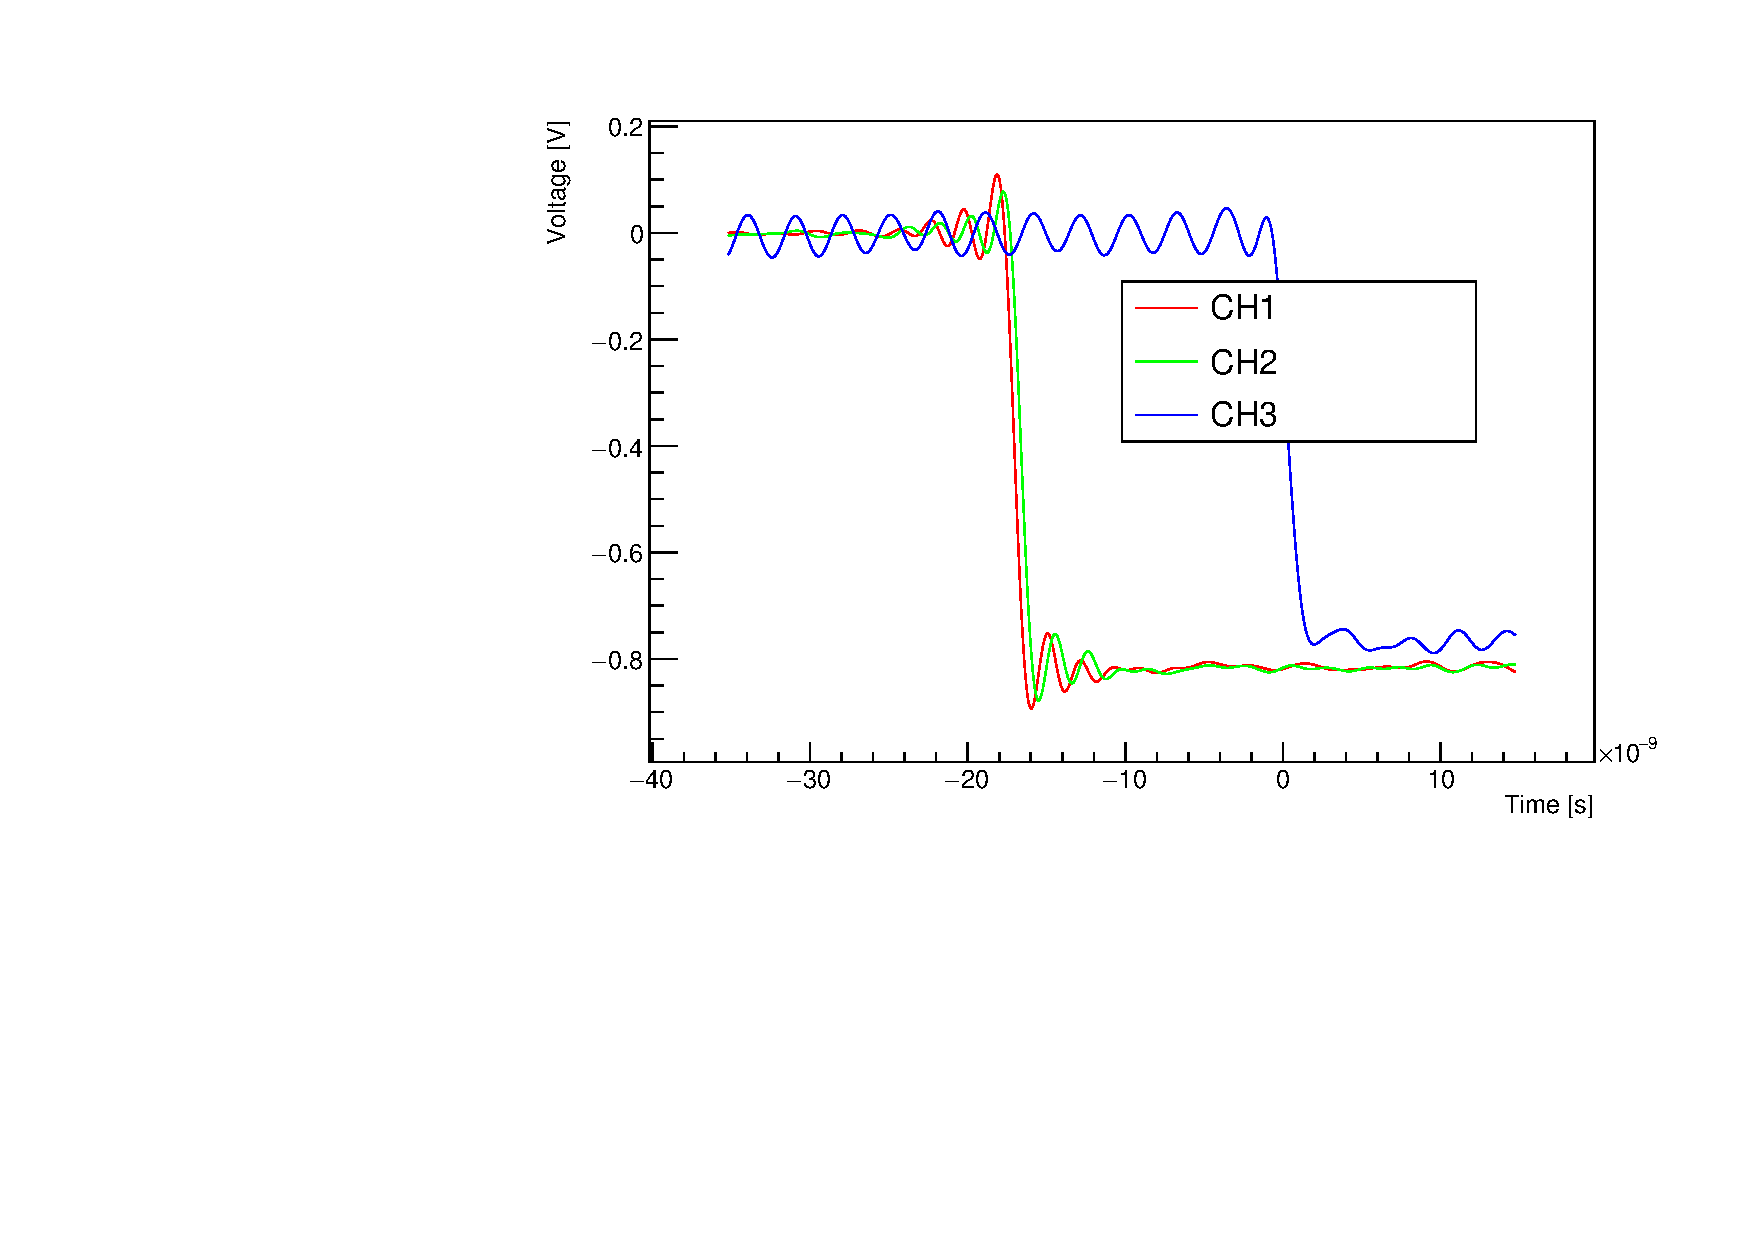
\includegraphics[width=0.9\textwidth]{../../ExperimentData/muspeed/muspeed/muspeed0.pdf}
\caption{典型信号}
\end{figure}
\end{column}

\begin{column}{0.5\columnwidth}
\begin{figure}[htbp]
\centering
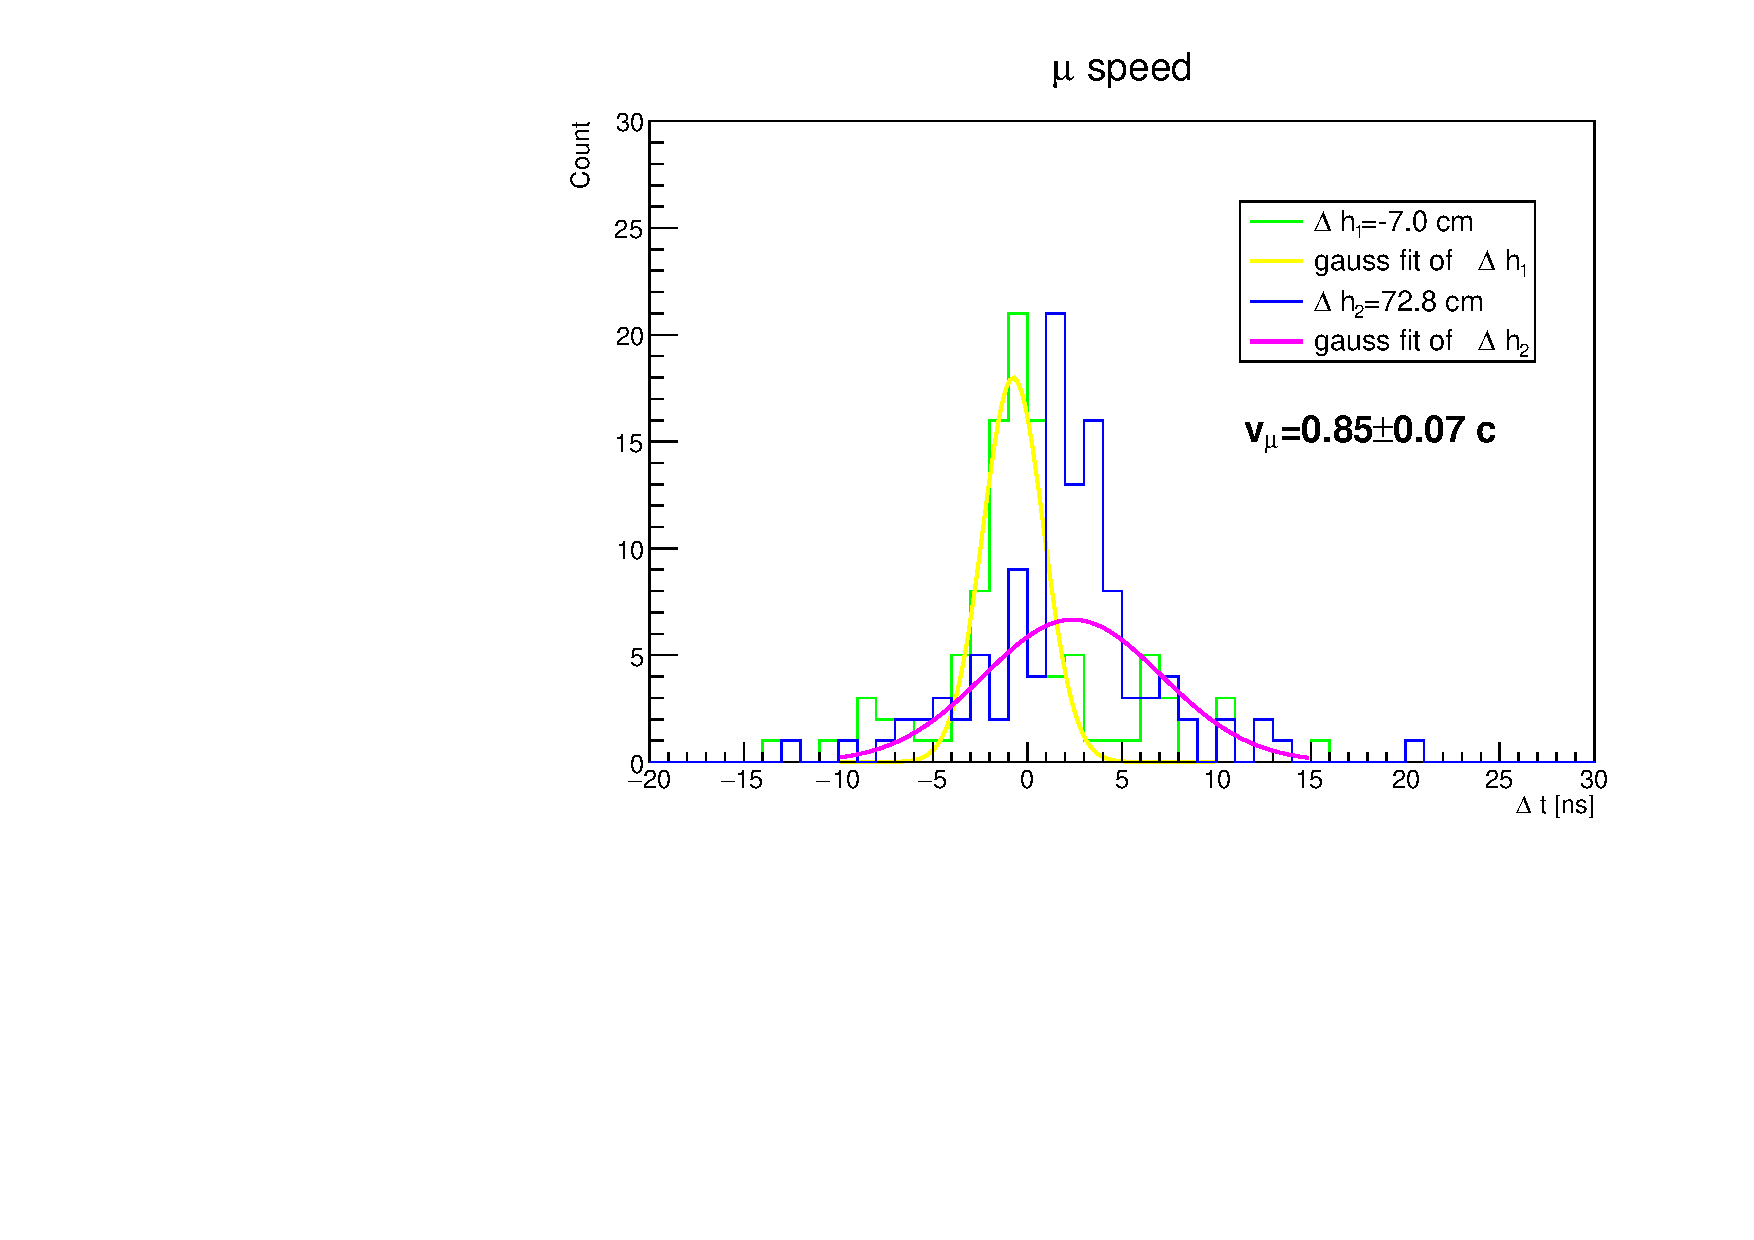
\includegraphics[width=0.9\textwidth]{../../mu/muspeed/muspeed.pdf}
\caption{\(\mu\) 速度}
\end{figure}
\end{column}
\end{columns}
\end{frame}

\section{总结}
\label{sec:orgd387d5d}
\begin{frame}[label={sec:org1d3c423}]{总结}
\begin{enumerate}
\item 在本学期的实验中, 我们对 \(\mu\) 和闪烁体的一些性质有了较好的理解, 对实验装置尤其是示波器的使用以及甄别阈和符合的设置有了更好的掌握, 同时也熟悉了 ROOT 等数据分析工具.
\item 实验中我们完成了:
\begin{itemize}
\item 电子学噪声, 暗噪声, \(\mu\) 信号的观察, 区分与计数率测量;
\item 余波的观察, 计数率与幅值测量;
\item 单光子电荷测量与能量刻度;
\item 衰减长度测量;
\item \(\mu\) 寿命测量;
\item Michel 电子能谱测量;
\item \(\mu\) 飞行时间测量.
\end{itemize}
\item 本实验的所有数据, 代码和报告可见 \url{https://github.com/Grant-S-Z/CosmicRayExperiment} , 敬请指正.
\end{enumerate}
\end{frame}
\end{document}